\begin{tikzpicture}

\GraphInit[vstyle=Classic]

\Vertex[Lpos=-90, x=0, y=0, L=$p_{1}$]{p1};
\Vertex[Lpos=-90, x=2, y=0, L=$p_{2}$]{p2};
\Vertex[Lpos=-90, x=4, y=0, L=$p_{3}$]{p3};
\Vertex[Lpos=-90, x=6, y=0, L=$p_{4}$]{p4};
\Vertex[Lpos=-90, x=8, y=0, L=$p_{t}$]{pt};
\Vertex[Lpos=-90, x=10, y=0, L=$p_{t + 1}$]{ptp1};
\Vertex[Lpos=-90, x=12, y=0, L=$p_{t + 2}$]{ptp2};
% https://tex.stackexchange.com/questions/265780/invisible-vertices-with-tkz-graph
\Vertex[empty,x=14, y=0]{p};

\Edge[style ={-},label={$a_{1}$},labelstyle={above}]({p1})({p2})
\Edge[style ={draw=none},label={$(a_{2})$},labelstyle={below}]({p1})({p2})
\Edge[style ={-},label={$a_{2}$},labelstyle={above}]({p2})({p3})
\Edge[style ={draw=none},label={$(a_{1})$},labelstyle={below}]({p2})({p3})
\Edge[style ={-},label={$a_{1}$},labelstyle={above}]({p3})({p4})
\Edge[style ={draw=none},label={$(a_{2})$},labelstyle={below}]({p3})({p4})
\Edge[style ={-},label={$a_{2}$},labelstyle={above}]({p4})({pt})
\Edge[style ={draw=none},label={$(a_{1})$},labelstyle={below}]({p4})({pt})
\Edge[style ={-},label={$a_{3}$},labelstyle={above}]({pt})({ptp1})
\Edge[style ={-},label={$a_{4}$},labelstyle={above}]({ptp1})({ptp2})
\Edge[style ={-},label={},labelstyle={above}]({ptp2})({p})

\end{tikzpicture}
